\documentclass[]{article}
\usepackage{lmodern}
\usepackage{amssymb,amsmath}
\usepackage{ifxetex,ifluatex}
\usepackage{fixltx2e} % provides \textsubscript
\ifnum 0\ifxetex 1\fi\ifluatex 1\fi=0 % if pdftex
  \usepackage[T1]{fontenc}
  \usepackage[utf8]{inputenc}
\else % if luatex or xelatex
  \ifxetex
    \usepackage{mathspec}
  \else
    \usepackage{fontspec}
  \fi
  \defaultfontfeatures{Ligatures=TeX,Scale=MatchLowercase}
\fi
% use upquote if available, for straight quotes in verbatim environments
\IfFileExists{upquote.sty}{\usepackage{upquote}}{}
% use microtype if available
\IfFileExists{microtype.sty}{%
\usepackage{microtype}
\UseMicrotypeSet[protrusion]{basicmath} % disable protrusion for tt fonts
}{}
\usepackage[margin=1in]{geometry}
\usepackage{hyperref}
\hypersetup{unicode=true,
            pdftitle={Lab 4},
            pdfauthor={Jonathan Ifegunni},
            pdfborder={0 0 0},
            breaklinks=true}
\urlstyle{same}  % don't use monospace font for urls
\usepackage{color}
\usepackage{fancyvrb}
\newcommand{\VerbBar}{|}
\newcommand{\VERB}{\Verb[commandchars=\\\{\}]}
\DefineVerbatimEnvironment{Highlighting}{Verbatim}{commandchars=\\\{\}}
% Add ',fontsize=\small' for more characters per line
\usepackage{framed}
\definecolor{shadecolor}{RGB}{248,248,248}
\newenvironment{Shaded}{\begin{snugshade}}{\end{snugshade}}
\newcommand{\KeywordTok}[1]{\textcolor[rgb]{0.13,0.29,0.53}{\textbf{#1}}}
\newcommand{\DataTypeTok}[1]{\textcolor[rgb]{0.13,0.29,0.53}{#1}}
\newcommand{\DecValTok}[1]{\textcolor[rgb]{0.00,0.00,0.81}{#1}}
\newcommand{\BaseNTok}[1]{\textcolor[rgb]{0.00,0.00,0.81}{#1}}
\newcommand{\FloatTok}[1]{\textcolor[rgb]{0.00,0.00,0.81}{#1}}
\newcommand{\ConstantTok}[1]{\textcolor[rgb]{0.00,0.00,0.00}{#1}}
\newcommand{\CharTok}[1]{\textcolor[rgb]{0.31,0.60,0.02}{#1}}
\newcommand{\SpecialCharTok}[1]{\textcolor[rgb]{0.00,0.00,0.00}{#1}}
\newcommand{\StringTok}[1]{\textcolor[rgb]{0.31,0.60,0.02}{#1}}
\newcommand{\VerbatimStringTok}[1]{\textcolor[rgb]{0.31,0.60,0.02}{#1}}
\newcommand{\SpecialStringTok}[1]{\textcolor[rgb]{0.31,0.60,0.02}{#1}}
\newcommand{\ImportTok}[1]{#1}
\newcommand{\CommentTok}[1]{\textcolor[rgb]{0.56,0.35,0.01}{\textit{#1}}}
\newcommand{\DocumentationTok}[1]{\textcolor[rgb]{0.56,0.35,0.01}{\textbf{\textit{#1}}}}
\newcommand{\AnnotationTok}[1]{\textcolor[rgb]{0.56,0.35,0.01}{\textbf{\textit{#1}}}}
\newcommand{\CommentVarTok}[1]{\textcolor[rgb]{0.56,0.35,0.01}{\textbf{\textit{#1}}}}
\newcommand{\OtherTok}[1]{\textcolor[rgb]{0.56,0.35,0.01}{#1}}
\newcommand{\FunctionTok}[1]{\textcolor[rgb]{0.00,0.00,0.00}{#1}}
\newcommand{\VariableTok}[1]{\textcolor[rgb]{0.00,0.00,0.00}{#1}}
\newcommand{\ControlFlowTok}[1]{\textcolor[rgb]{0.13,0.29,0.53}{\textbf{#1}}}
\newcommand{\OperatorTok}[1]{\textcolor[rgb]{0.81,0.36,0.00}{\textbf{#1}}}
\newcommand{\BuiltInTok}[1]{#1}
\newcommand{\ExtensionTok}[1]{#1}
\newcommand{\PreprocessorTok}[1]{\textcolor[rgb]{0.56,0.35,0.01}{\textit{#1}}}
\newcommand{\AttributeTok}[1]{\textcolor[rgb]{0.77,0.63,0.00}{#1}}
\newcommand{\RegionMarkerTok}[1]{#1}
\newcommand{\InformationTok}[1]{\textcolor[rgb]{0.56,0.35,0.01}{\textbf{\textit{#1}}}}
\newcommand{\WarningTok}[1]{\textcolor[rgb]{0.56,0.35,0.01}{\textbf{\textit{#1}}}}
\newcommand{\AlertTok}[1]{\textcolor[rgb]{0.94,0.16,0.16}{#1}}
\newcommand{\ErrorTok}[1]{\textcolor[rgb]{0.64,0.00,0.00}{\textbf{#1}}}
\newcommand{\NormalTok}[1]{#1}
\usepackage{graphicx,grffile}
\makeatletter
\def\maxwidth{\ifdim\Gin@nat@width>\linewidth\linewidth\else\Gin@nat@width\fi}
\def\maxheight{\ifdim\Gin@nat@height>\textheight\textheight\else\Gin@nat@height\fi}
\makeatother
% Scale images if necessary, so that they will not overflow the page
% margins by default, and it is still possible to overwrite the defaults
% using explicit options in \includegraphics[width, height, ...]{}
\setkeys{Gin}{width=\maxwidth,height=\maxheight,keepaspectratio}
\IfFileExists{parskip.sty}{%
\usepackage{parskip}
}{% else
\setlength{\parindent}{0pt}
\setlength{\parskip}{6pt plus 2pt minus 1pt}
}
\setlength{\emergencystretch}{3em}  % prevent overfull lines
\providecommand{\tightlist}{%
  \setlength{\itemsep}{0pt}\setlength{\parskip}{0pt}}
\setcounter{secnumdepth}{0}
% Redefines (sub)paragraphs to behave more like sections
\ifx\paragraph\undefined\else
\let\oldparagraph\paragraph
\renewcommand{\paragraph}[1]{\oldparagraph{#1}\mbox{}}
\fi
\ifx\subparagraph\undefined\else
\let\oldsubparagraph\subparagraph
\renewcommand{\subparagraph}[1]{\oldsubparagraph{#1}\mbox{}}
\fi

%%% Use protect on footnotes to avoid problems with footnotes in titles
\let\rmarkdownfootnote\footnote%
\def\footnote{\protect\rmarkdownfootnote}

%%% Change title format to be more compact
\usepackage{titling}

% Create subtitle command for use in maketitle
\newcommand{\subtitle}[1]{
  \posttitle{
    \begin{center}\large#1\end{center}
    }
}

\setlength{\droptitle}{-2em}

  \title{Lab 4}
    \pretitle{\vspace{\droptitle}\centering\huge}
  \posttitle{\par}
    \author{Jonathan Ifegunni}
    \preauthor{\centering\large\emph}
  \postauthor{\par}
      \predate{\centering\large\emph}
  \postdate{\par}
    \date{September 16, 2018}


\begin{document}
\maketitle

\section{Task 1}\label{task-1}

\begin{Shaded}
\begin{Highlighting}[]
\KeywordTok{getwd}\NormalTok{()}
\end{Highlighting}
\end{Shaded}

\begin{verbatim}
## [1] "C:/Users/obi4m/OneDrive/Desktop/LAB4"
\end{verbatim}

\section{Task 2}\label{task-2}

\begin{Shaded}
\begin{Highlighting}[]
\CommentTok{# read in SPRUCE.csv data file}
\NormalTok{spruce.df =}\StringTok{ }\KeywordTok{read.csv}\NormalTok{(}\StringTok{"SPRUCE.csv"}\NormalTok{)}
\CommentTok{# display last six lines}
\KeywordTok{tail}\NormalTok{(spruce.df)}
\end{Highlighting}
\end{Shaded}

\begin{verbatim}
##    BHDiameter Height
## 31       17.7   19.9
## 32       20.7   19.4
## 33       21.0   20.4
## 34       13.3   15.5
## 35       15.9   17.6
## 36       22.9   19.2
\end{verbatim}

\section{Task 3}\label{task-3}

\subsection{A}\label{a}

\begin{Shaded}
\begin{Highlighting}[]
\KeywordTok{library}\NormalTok{(s20x)}
\KeywordTok{trendscatter}\NormalTok{(Height}\OperatorTok{~}\NormalTok{BHDiameter,}\DataTypeTok{f=}\FloatTok{0.5}\NormalTok{,}\DataTypeTok{data=}\NormalTok{spruce.df)}
\end{Highlighting}
\end{Shaded}

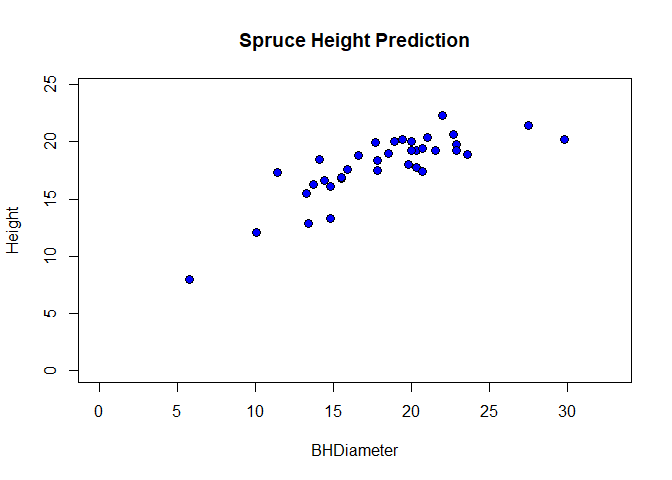
\includegraphics{lab4_files/figure-latex/unnamed-chunk-3-1.pdf}

\subsection{B}\label{b}

\begin{Shaded}
\begin{Highlighting}[]
\CommentTok{# make linear model  of spruce data}
\NormalTok{spruce.lm=}\KeywordTok{lm}\NormalTok{(Height}\OperatorTok{~}\NormalTok{BHDiameter,}\DataTypeTok{data=}\NormalTok{spruce.df)}
\KeywordTok{summary}\NormalTok{(spruce.lm)}
\end{Highlighting}
\end{Shaded}

\begin{verbatim}
## 
## Call:
## lm(formula = Height ~ BHDiameter, data = spruce.df)
## 
## Residuals:
##     Min      1Q  Median      3Q     Max 
## -3.9394 -0.9763  0.2829  0.9950  2.6644 
## 
## Coefficients:
##             Estimate Std. Error t value Pr(>|t|)    
## (Intercept)  9.14684    1.12131   8.157 1.63e-09 ***
## BHDiameter   0.48147    0.05967   8.069 2.09e-09 ***
## ---
## Signif. codes:  0 '***' 0.001 '**' 0.01 '*' 0.05 '.' 0.1 ' ' 1
## 
## Residual standard error: 1.678 on 34 degrees of freedom
## Multiple R-squared:  0.6569, Adjusted R-squared:  0.6468 
## F-statistic:  65.1 on 1 and 34 DF,  p-value: 2.089e-09
\end{verbatim}

\subsection{C}\label{c}

\begin{Shaded}
\begin{Highlighting}[]
\CommentTok{#residuals  created from the linear model object}
\NormalTok{height.res=}\KeywordTok{residuals}\NormalTok{(spruce.lm)}
\CommentTok{#fitted values made from the linear model object}
\NormalTok{height.fit=}\KeywordTok{fitted}\NormalTok{(spruce.lm)}
\CommentTok{# make linear model  of spruce data}
\KeywordTok{plot}\NormalTok{(height.fit,height.res)}
\end{Highlighting}
\end{Shaded}

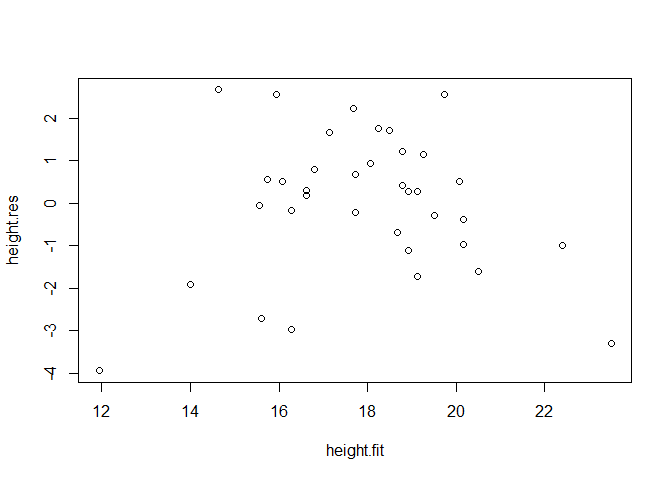
\includegraphics{lab4_files/figure-latex/unnamed-chunk-5-1.pdf}

\begin{Shaded}
\begin{Highlighting}[]
\CommentTok{# Put a lowess smoother through res vs fitted}
\KeywordTok{trendscatter}\NormalTok{( height.fit,height.res)}
\end{Highlighting}
\end{Shaded}

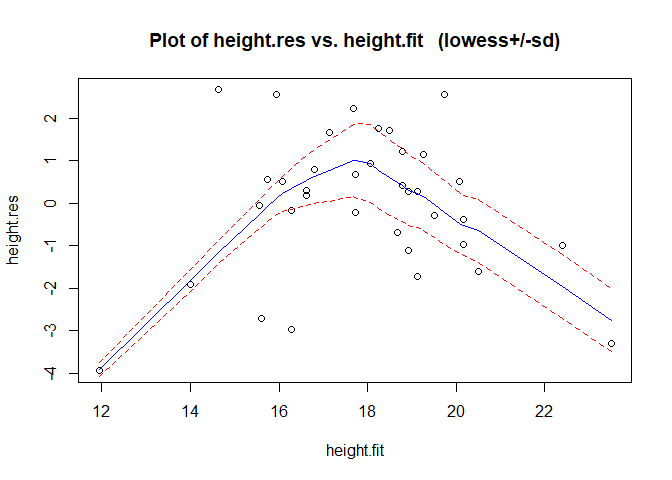
\includegraphics{lab4_files/figure-latex/unnamed-chunk-5-2.pdf}

\subsection{D}\label{d}

\begin{quote}
What shape is seen in the plot? Compare it with the curve made with the
trendscatter function (second line after Task3).
\end{quote}

\begin{quote}
We can see clear elements of the original signal in the residual plot.
This implies that the model has not all the points in the original data
set.
\end{quote}

\subsection{E}\label{e}

\begin{Shaded}
\begin{Highlighting}[]
\CommentTok{# Make quick plot of residuals}
\KeywordTok{windows}\NormalTok{()}
\KeywordTok{plot}\NormalTok{(spruce.lm, }\DataTypeTok{which =}\DecValTok{1}\NormalTok{)}
\end{Highlighting}
\end{Shaded}

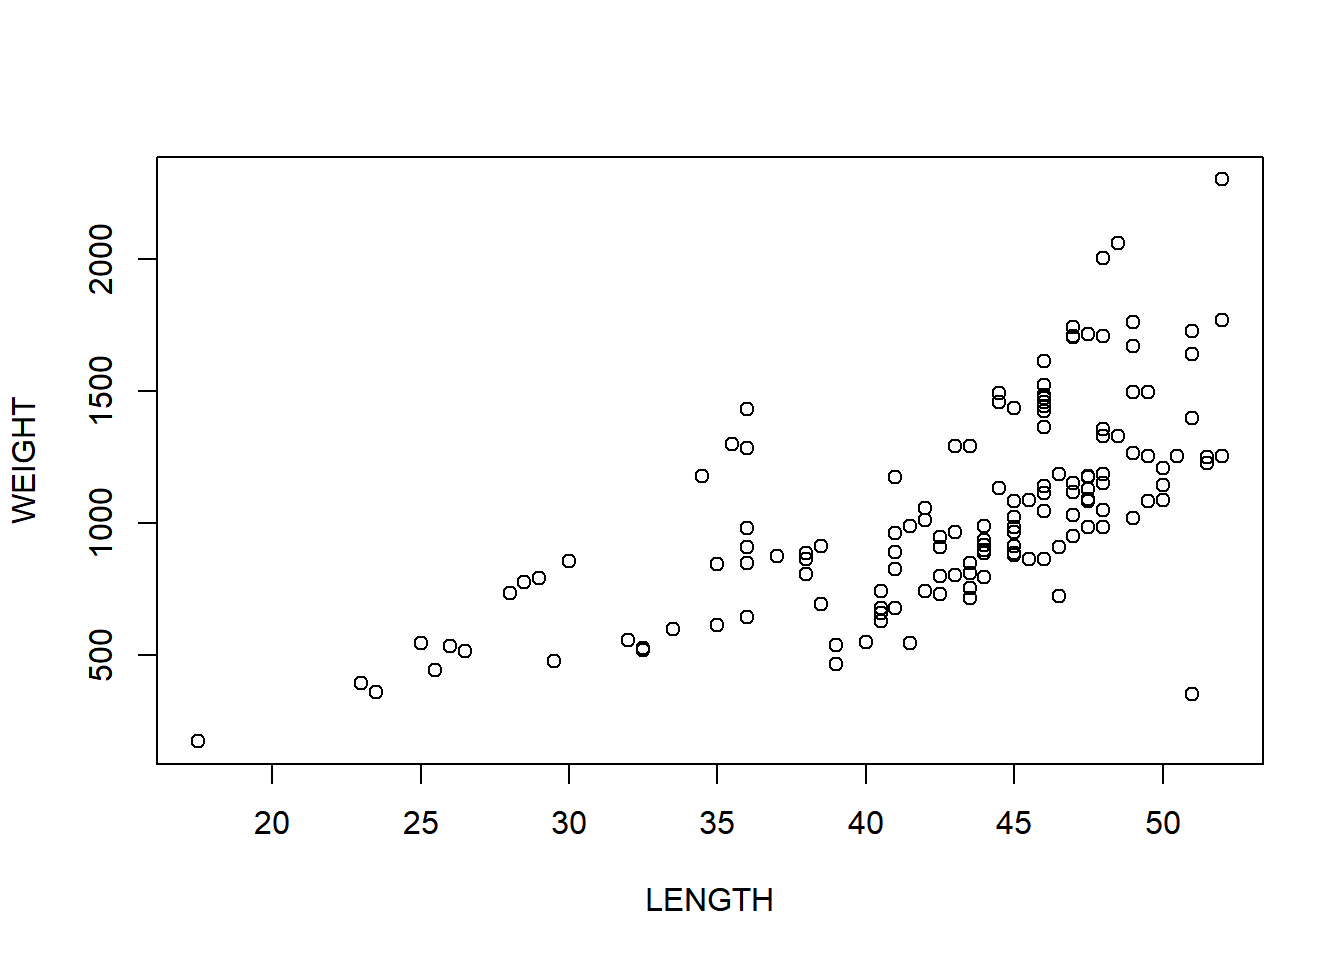
\includegraphics{lab4_files/figure-latex/unnamed-chunk-6-1.pdf}

\subsection{F}\label{f}

\begin{quote}
Check normality using the s20x function normcheck(). Please note that
you may need to add an additional option to show the Shapiro-Wilk test
(use ?normcheck )
\end{quote}

\begin{Shaded}
\begin{Highlighting}[]
\CommentTok{# Two plots testing normality}
\KeywordTok{windows}\NormalTok{()}
\KeywordTok{normcheck}\NormalTok{(spruce.lm,}\DataTypeTok{shapiro.wilk =} \OtherTok{TRUE}\NormalTok{)}
\end{Highlighting}
\end{Shaded}

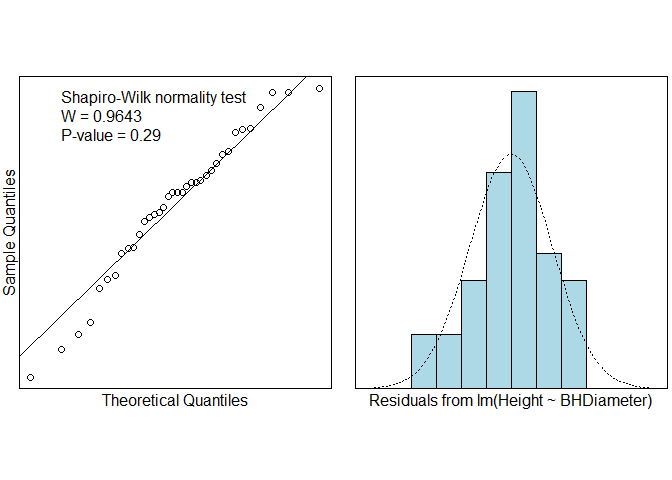
\includegraphics{lab4_files/figure-latex/unnamed-chunk-7-1.pdf}


\end{document}
